\chapter{The sPHENIX Project}
\label{chap:project}

The sPHENIX detector is being realized via several projects that are
coordinated under a common project management structure.  There are
the elements of the original DOE MIE --- the 1.5~T BaBar
superconducting solenoid, the outer hadronic calorimeter (oHCal), the
central rapidity portion of electromagnetic calorimeter (EMCal)
covering $|\eta| < 0.85$, the time projection chamber (TPC), and their
associated readout electronics and services.  A silicon strip tracker
(INTT) is being provied by RIKEN.  Additional tungsten/scintillating
fiber blocks extending the coverage of the EMCal to $|\eta| < 1.1$ are
being provided by a consortium of Chinese collaborating institutions.
The inner longitudinal section of the hadronic calorimeter (iHCal) and
the silicon pixel vertex detector (MVTX) are being pursued as BNL
capital projects.  A quartz \v{C}erenkov minimum bias detector,
originally built by Hiroshima University for the PHENIX experiment, is
being repurposed for use in sPHENIX.  There are also BNL funded
projects to upgrade the infrastructure at IP8 and to integrate and
install the sPHENIX detector into the IP.  A labeled depiction of the
sPHENIX detector can be seen in Fig.~\ref{fig:sPHENIX}.

\section{Project timeline}
\label{sec:timeline}

The sPHENIX MIE received CD-1/3A approval in August 2018.  A memo from DOE 

\section{Elements of the Project}
\label{sec:elements}

\begin{figure}[hbt!]
  \centering
  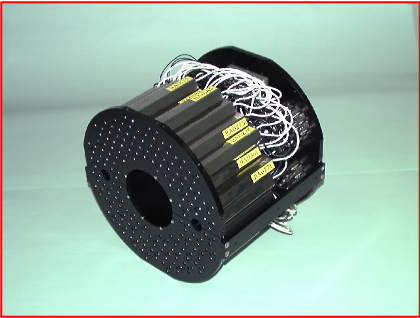
\includegraphics{mbd}
  \caption{The minimum bias detector. Originally built by Hiroshima University for HENIX, being reused for sPHENIX. }
  \label{fig:mbd}
\end{figure}

\begin{figure}[hbt!]
  \centering
  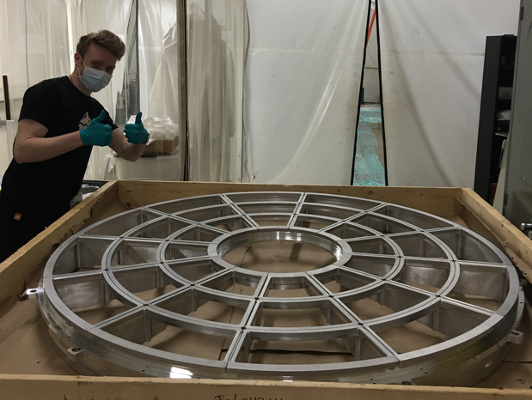
\includegraphics{wagonwheel}
  \caption{The structure --- the ``wagon wheel'' ---  which supports
    the TPC field cages, the GEMs, the readout electronics and all the
    services.  It is milled from a single billet of aluminum in order to
    eliminate joints which could allow seepage and complicate
    controlling the purity of the contained gas. }
  \label{fig:wagonwheel}
\end{figure}

\begin{figure}[hbt!]
  \centering
  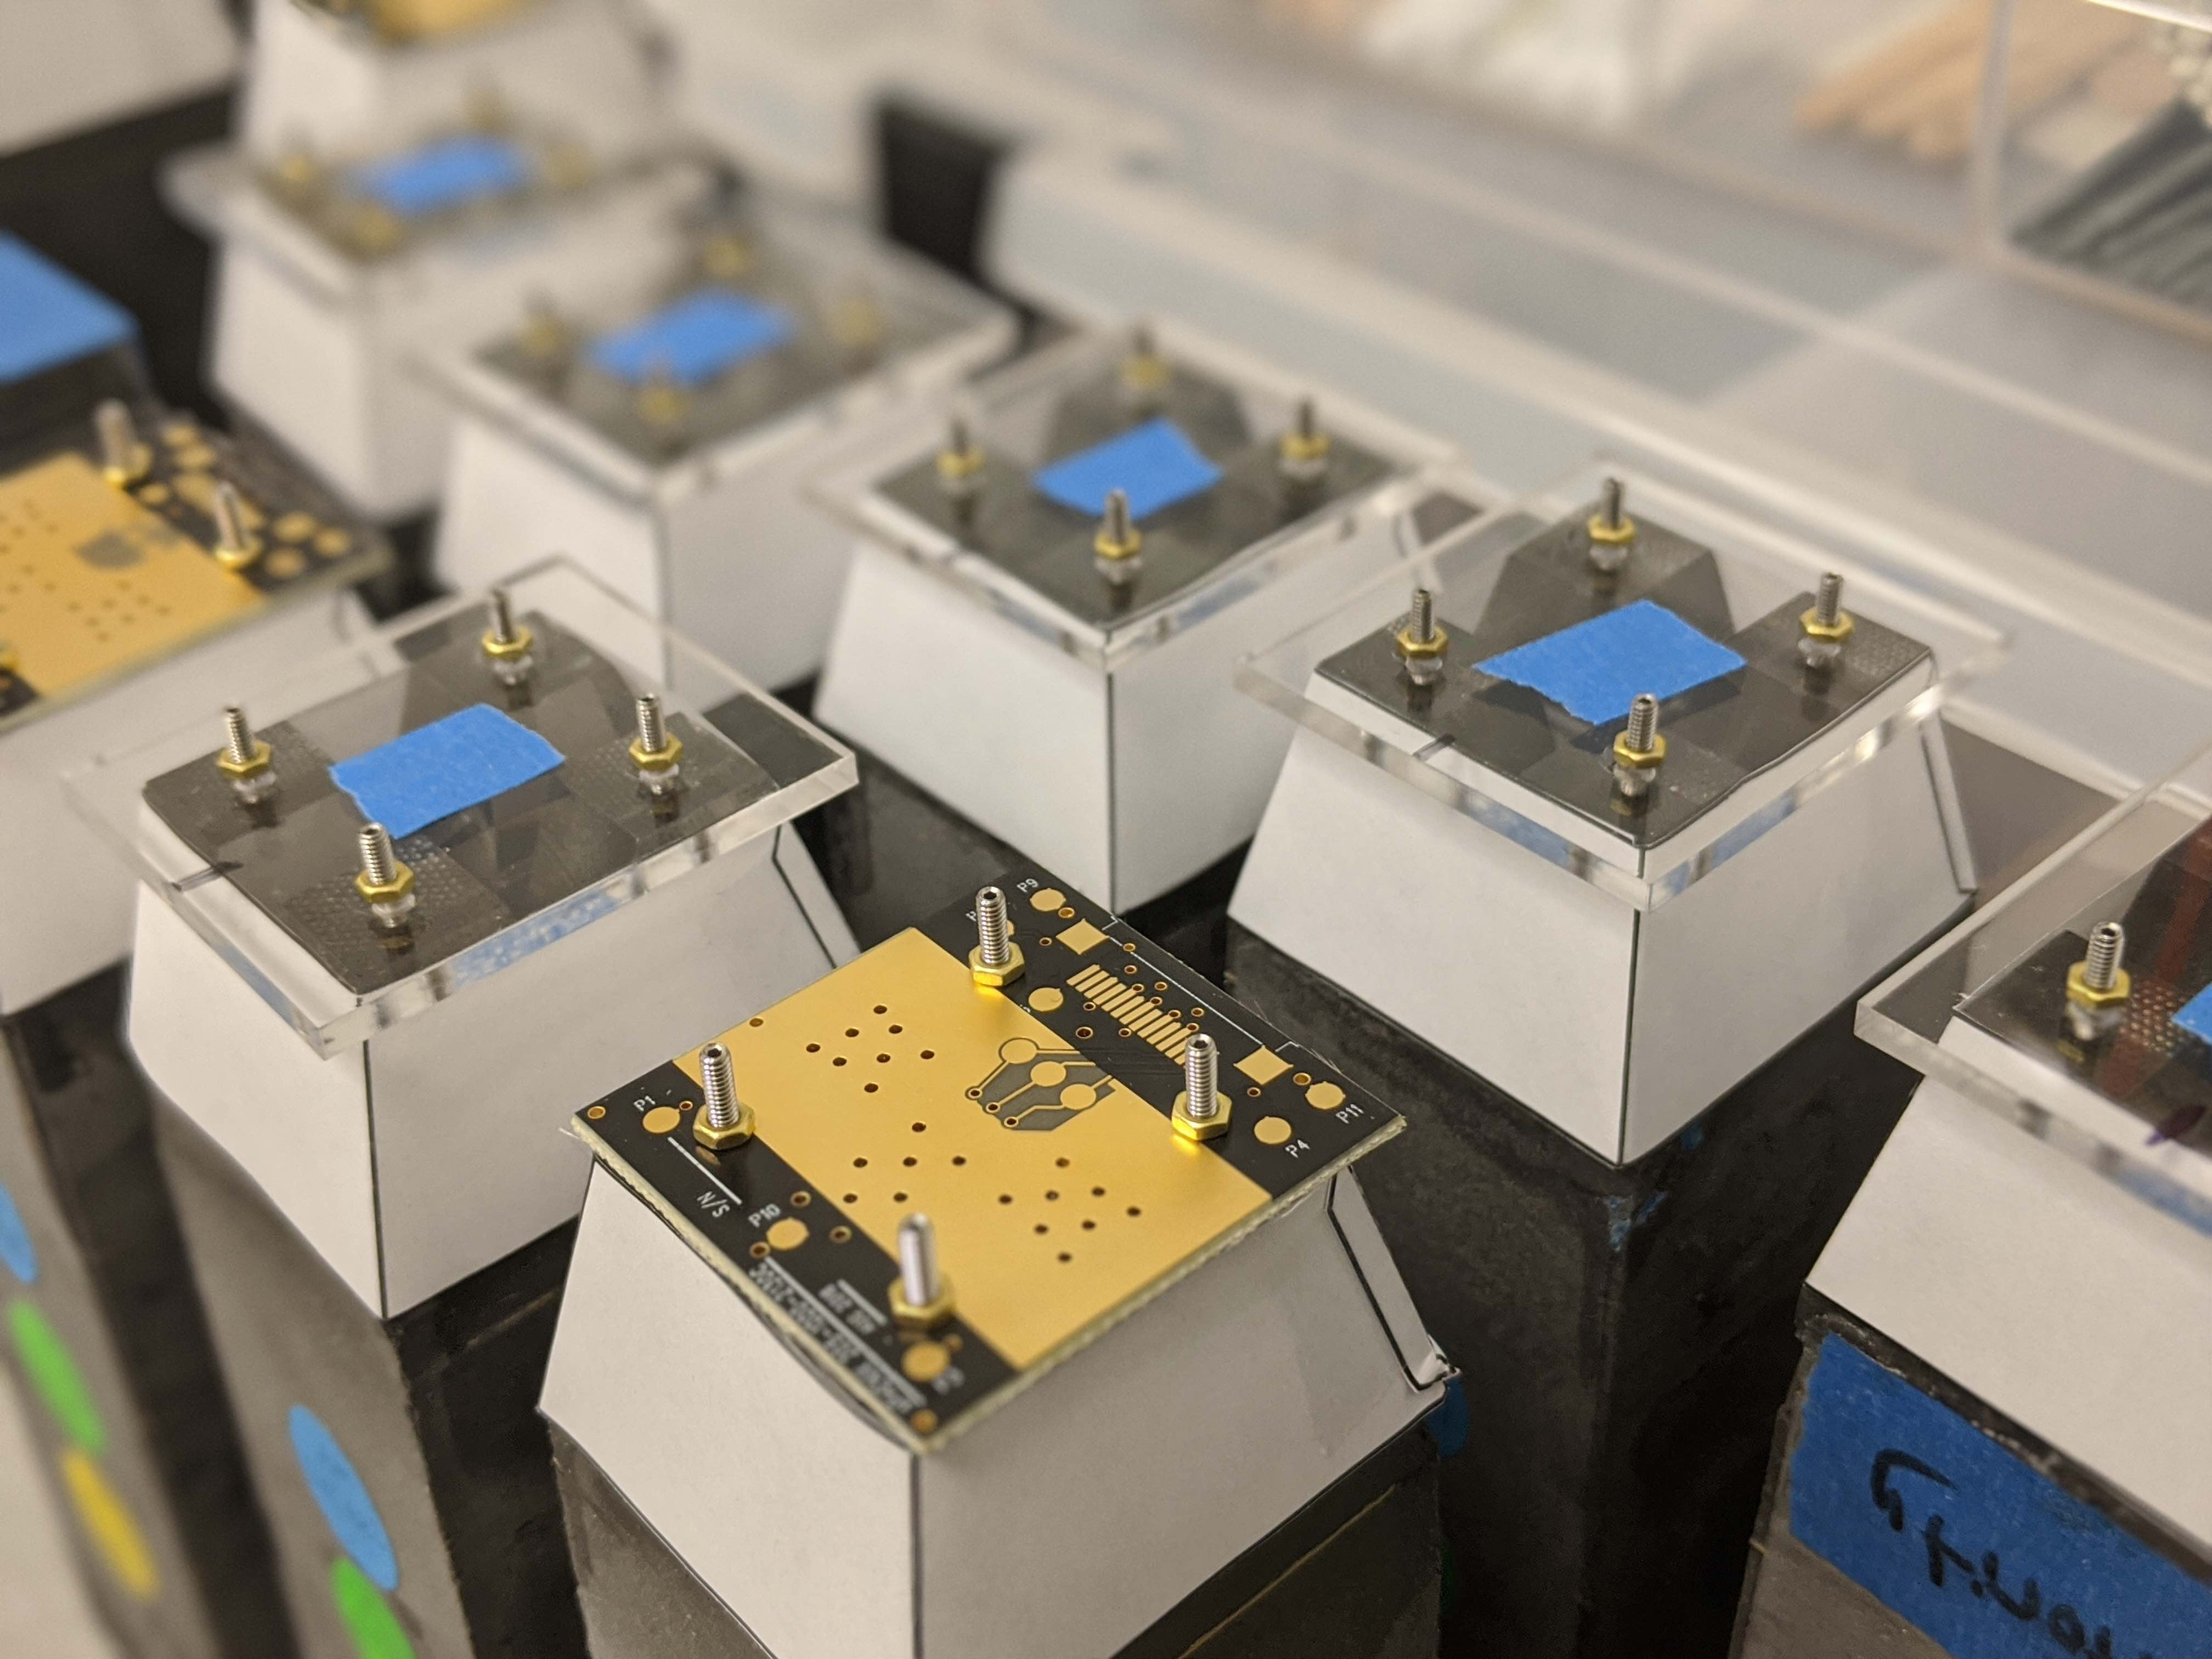
\includegraphics[width=0.45\linewidth]{emcalblocks}
  \hfill
  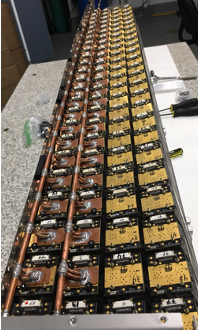
\includegraphics[width=0.45\linewidth]{sector0}
  \caption{The EMCal blocks and the assembled EMCal Sector ``0''.}
  \label{fig:emcal}
\end{figure}




\section{Progress since last PAC}
\label{sec:progress}

The sPHENIX MIE was granted PD-2/3 on September 20, 2019.

\begin{figure}[!hbt]
 \begin{center}
%    \includegraphics[width=0.7\linewidth]{}
        \caption{\label{fig:ohcal}All 32 sectors of the oHCal have
        been delivered and are in Bldg. 912.  A few of the sectors have
        been instrumented.}
 \end{center}
\end{figure}

\begin{figure}[!hbt]
 \begin{center}
%    \includegraphics[width=0.7\linewidth]{}
        \caption{\label{fig:ihcal}Prototype of the iHCal.  The
        construction of this is being pursued as a BNL capital project.}
 \end{center}
\end{figure}

\begin{figure}[!hbt]
 \begin{center}
%    \includegraphics[width=0.7\linewidth]{}
        \caption{\label{fig:tpc}Photos of the TPC under construction
        at Stony Brook University.}
 \end{center}
\end{figure}

\begin{figure}[!hbt]
 \begin{center}
%    \includegraphics[width=0.7\linewidth]{}
        \caption{\label{fig:intt}Staves of the silicon strip detector (INTT).}
 \end{center}
\end{figure}

\begin{figure}[!hbt]
 \begin{center}
%    \includegraphics[width=0.7\linewidth]{}
        \caption{\label{fig:mvtx}Construction photos of the MVTX.}
 \end{center}
\end{figure}


Computing needs.

Effects of COVID-19.

Relationship to EIC.

Prospects for being ready for data taking in 2023.

